% Trimmed 2026-09-22 (round 2): overview cut to what Intro P4 does not say; lifting paragraph, 3.2 tail and
% 3.4 opening/closing compressed; the four >30-word sentences split.
% Compressed 2026-09-21 (page budget, items A4/A5): closed-form rollout inlined; the two
% execution/replanning paragraphs of 3.3 merged; the duplicate learned-lifting paragraph of 3.2 removed;
% the ARX sentence of 3.1 split. Equations (4)(5)(6)(8)(9) unchanged.
\section{Method}
\label{sec:method}

KOMPAS consists of an offline dynamics model, fit on recorded attribute
readings, and an online controller that plans in that model and
replans after every reply (receding horizon). The frozen LLM $p_\theta$ is never updated, and candidate evaluation
requires no additional query to it. Figure~\ref{fig:method} summarizes the
pipeline; the first three subsections follow it and \S\ref{sec:prediction_control_bound} gives the guarantee.

\begin{figure}[t]
    \centering
    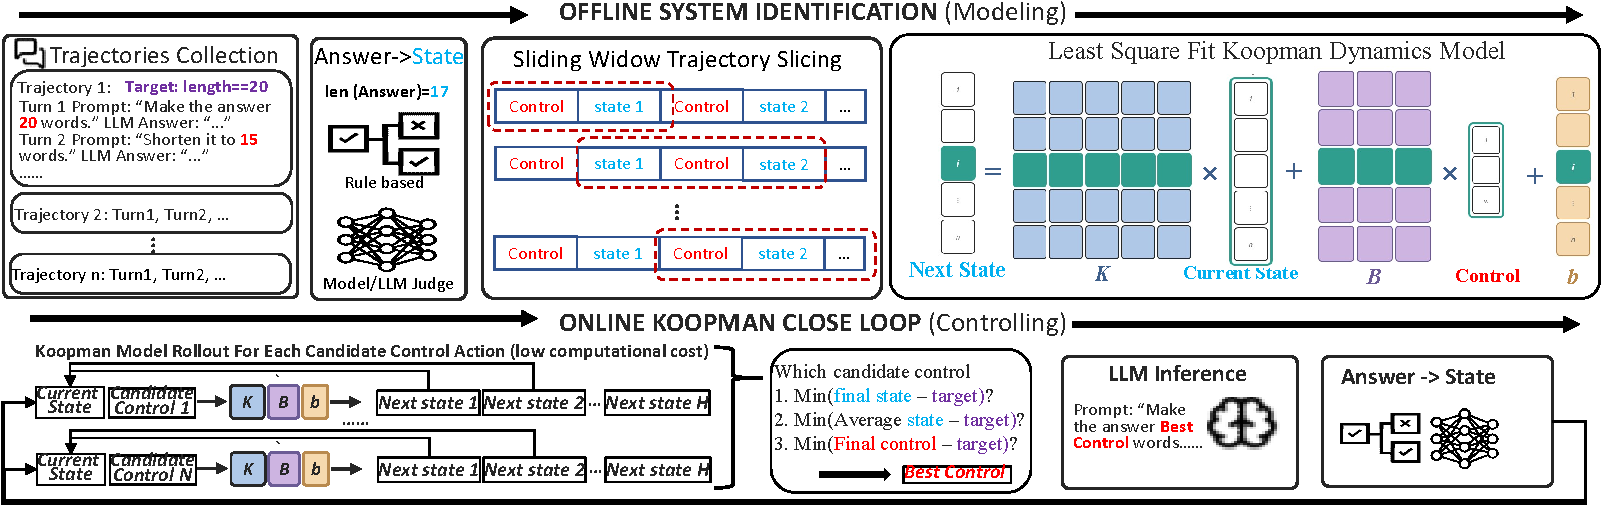
\includegraphics[width=\textwidth]{figs/MethodCropped.pdf}
    \caption{
    Overview of KOMPAS. Top, offline fitting: recorded trajectories
    are mapped by the verifier $V$ to readings, a sliding window
    forms the state $s_t$, and the affine Koopman model is fit by least squares.
    Bottom, online closed loop: candidate commands $c_t$ are rolled forward
    through the dynamics model, scored against the reference $r$, and the best one is
    sent through the prompting protocol as $u_t$; the next reading is shifted
    into the state and the selection repeats.
    }
    \label{fig:method}
\end{figure}


\subsection{Observable-State Koopman Dynamics}
\label{sec:model}

The controller does not model text. Each completed response $o_t$
is mapped by the task-specific verifier $V$ from
Section~\ref{sec:problem_modeling} to a scalar attribute $y_t=V(o_t)$.
The particular definition of $V$ depends on the task and is given in the
experimental setup; the dynamics model uses only the resulting scalar
readings.

A single reading generally does not retain enough temporal context to
predict the next one. The same value $y_t$, for example, may occur along an
increasing or decreasing trajectory and therefore lead to different future
responses. We represent this short-term history with delay coordinates
$s_t=[\,y_t,\,y_{t-1},\,\ldots,\,y_{t-L}\,]^{\top}\in\mathbb{R}^{L+1}$ with readout $y_t=Cs_t$,\label{eq:memory_state}  % inlined 2026-09-23 (page budget); label kept for the contract lattice
where $L\geq 1$ is the number of previous readings retained and
$C=[1,0,\ldots,0]$ reads the current attribute from the state. We use
$s_t$ as a finite-memory stand-in for the part of the dialogue history that
predicts the attribute, not as a summary of the dialogue text itself.

The controller acts through a scalar command rather than over the
space of text strings. A fixed prompting protocol maps a command
$c_t\in\mathcal{C}\subseteq\mathbb{R}$ to the textual instruction
$u_t=\mathcal{P}(x,\mathcal{H}_t,c_t)$. Thus, after fixing
$\mathcal{P}$, the controlled interaction can be viewed at the attribute
level as a transition from $(s_t,c_t)$ to $s_{t+1}$.

This controlled transition induces a command-conditioned Koopman operator
on observables. For an observable $f$, we define
$(\mathcal{K}_c f)(s)
=
\mathbb{E}[f(s_{t+1})\mid s_t=s,c_t=c]$.
The operator is linear in $f$ even when the underlying prompt--response
interaction is nonlinear. We use the delay coordinates in $s_t$ as a finite
dictionary of observables, that is, the feature set the linear model acts on.
The induced dynamics are approximated with the
affine model
\begin{equation}
    \widehat{s}_{t+1}
    =
    K s_t+B c_t+b,
    \qquad
    \widehat{y}_{t+1}
    =
    C\widehat{s}_{t+1}.
    \label{eq:koopman_model}
\end{equation}
Here $K\in\mathbb{R}^{(L+1)\times(L+1)}$ propagates the memory state,
$B\in\mathbb{R}^{(L+1)\times 1}$ captures the effect of the command, and
$b\in\mathbb{R}^{L+1}$ is a bias term. Sharing one transition matrix across
commands and letting the command enter through one linear channel are
modeling choices, not consequences of Koopman linearity. We do not assume
that the frozen LLM admits an exact finite-dimensional Koopman representation.

Koopman dynamics may also be defined on lifted coordinates $E_\phi(s_t)$:
a feature map applied to the window before the linear model, called a
lifting. Our reported predictor uses the identity lifting, that is, no
feature map; a learned lifting is kept as a comparison with its objective in
Appendix~\ref{app:A1_estimator}. The reported predictor is thus also a delay
regression with an exogenous input. The Koopman view places both dictionaries in one framework and
gives closed-form multi-step prediction.


\subsection{Offline Fitting (System Identification)}
\label{sec:learning}

We fit the dynamics model from recorded interaction trajectories. Sliding a
window of $L+1$ readings over a trajectory produces transition tuples
$(s_t,c_t,s_{t+1})$, where $c_t$ is the command applied before observing the
successor state.

Because $K$, $B$, and $b$ enter the one-step prediction linearly, the
identity-lifting model is estimated by least squares,
$(\widehat K,\widehat B,\widehat b)=\arg\min_{K,B,b}\sum_t\|s_{t+1}-(Ks_t+Bc_t+b)\|_2^2$.\label{eq:koopman_fit}  % inlined 2026-09-23 (page budget)
The fit is performed offline and does not modify the parameters $\theta$
of the target LLM. The learned dynamics can be trusted only on the
state--command combinations represented in the recorded trajectories.


\subsection{Receding-Horizon Prompt Control}
\label{sec:control_method}

At inference time, candidate commands are evaluated in the learned dynamics
rather than by querying the LLM. Let $\mathcal{C}_t\subseteq\mathcal{C}$ be
the finite set of candidate commands at step $t$; each $c\in\mathcal{C}_t$
is held fixed inside a hypothetical $H$-step rollout from the observed state
$s_t$. The predicted state obeys
$\widehat{s}_{t|t}(c)=s_t$ and
$\widehat{s}_{t+h|t}(c)
=
K\widehat{s}_{t+h-1|t}(c)+Bc+b$,
with
$\widehat y_{t+h|t}(c)=C\widehat{s}_{t+h|t}(c)$.

Because the transition is affine, the rollout has the closed form
$\widehat{s}_{t+h\mid t}(c)=K^h s_t+\sum_{j=0}^{h-1}K^j(Bc+b)$, so candidate
evaluation is linear propagation through the fitted model and adds no
call to $p_\theta$.

Each candidate is scored by the deviation of its predicted trajectory from
the desired attribute,
\begin{equation}
    \widehat{J}_t(c)
    =
    \sum_{h=1}^{H}
    w_h
    \left|
        \widehat y_{t+h\mid t}(c)-r
    \right|^2,
    \qquad
    c_t^\star
    \in
    \arg\min_{c\in\mathcal{C}_t}
    \widehat{J}_t(c),
    \quad
    w_h\geq 0.
    \label{eq:predictive_control}
\end{equation}
Here $\widehat{J}_t(c)$ is the predicted cost of holding candidate $c$, $w_h$
weights the horizon steps, and $c_t^\star$ is the selected command. Scoring the
whole predicted trajectory allows the selected command to differ from the
reference while the attribute is still moving toward it.

The controller executes only $c_t^\star$: it sends
$u_t=\mathcal{P}(x,\mathcal{H}_t,c_t^\star)$, measures $y_{t+1}=V(o_{t+1})$
from the actual response, shifts it into the memory state, and repeats the
selection from $s_{t+1}$. The held-command assumption applies only inside a
candidate's hypothetical rollout; the executed sequence is replanned after
every reply and may change command at every step.


\subsection{Why Prediction Accuracy Matters}
\label{sec:prediction_control_bound}

Predictive control is useful only when ranking candidates under the learned
dynamics model preserves their ranking under the true interaction, up to a bounded
error. The following result states this for the comparison among candidates,
each held for $H$ steps, at one control step.

For a candidate $c$, let $y_h^c$ denote the realized attribute after
$h$ further interactions under the same held command, and let
$J_t(c)=\sum_{h=1}^{H}w_h|y_h^c-r|^2$ be its realized trajectory cost.
Suppose the one-step state residual along candidate rollouts is bounded by
$\varepsilon_{\mathrm{dyn}}$, the readout residual is bounded by
$\varepsilon_{\mathrm{rec}}$, and the readout is Lipschitz on the region
visited by the rollouts. Then the $h$-step prediction error is bounded by
some $\Delta_h$, and the command selected by Eq.~(\ref{eq:predictive_control})
satisfies
$J_t(c_t^\star)\leq\min_{c\in\mathcal{C}_t} J_t(c)+2\delta_J$,\label{eq:selection_bound}  % inlined 2026-09-23 (page budget); A6 now refers to "the selection bound of Section 3.4"
where $\delta_J$ is the corresponding bound on the difference between
predicted and realized candidate costs. Appendix~\ref{app:A6_selection_bound}
gives the explicit forms of $\Delta_h$ and $\delta_J$ and the proof.

The result is local: it concerns candidate selection at one replanning step
and does not assert convergence of the closed loop. Its role is to link the
two objectives: more accurate rollouts bring the selected command closer to
the best command under the realized costs.